%% LyX 2.0.6 created this file.  For more info, see http://www.lyx.org/.
%% Do not edit unless you really know what you are doing.
\documentclass[twocolumn,english,aps,superscriptaddress,prl,showpacs]{revtex4}
\usepackage[T1]{fontenc}
\usepackage[latin9]{inputenc}
\setcounter{secnumdepth}{3}
\usepackage{amsmath}
\usepackage{amssymb}
\usepackage{graphicx}
\usepackage{esint}
\usepackage{color}

\makeatletter
%%%%%%%%%%%%%%%%%%%%%%%%%%%%%% Textclass specific LaTeX commands.
\@ifundefined{textcolor}{}
{%
 \definecolor{BLACK}{gray}{0}
 \definecolor{WHITE}{gray}{1}
 \definecolor{RED}{rgb}{1,0,0}
 \definecolor{GREEN}{rgb}{0,1,0}
 \definecolor{BLUE}{rgb}{0,0,1}
 \definecolor{CYAN}{cmyk}{1,0,0,0}
 \definecolor{MAGENTA}{cmyk}{0,1,0,0}
 \definecolor{YELLOW}{cmyk}{0,0,1,0}
}

%%%%%%%%%%%%%%%%%%%%%%%%%%%%%% User specified LaTeX commands.
\newcommand{\aualyb}{\mbox{Au}_{51}\mbox{Al}_{34}\mbox{Yb}_{15}}
\newcommand{\tk}{T_{\rm K}}
\newcommand{\tkt}{T_{\rm K}^{\rm typ}}
\newcommand{\tkm}{T_{\rm K}^{\rm min}}

\newcommand{\todo}[1]{{\color{red} {\bf [ToDo: #1]}}}
\newcommand{\define}{\ensuremath{ \overset{\text{def}}{=} }}

% differential element
\renewcommand{\d}[1]{\mathrm{d}#1}

% similar symbol with a limit underneath
\newcommand{\simlim}[2]{\ensuremath{ \underset{#1 \rightarrow #2}{\sim} }}

\newcommand{\om}{\ensuremath{\omega}}
\newcommand{\lb}{\ensuremath{\overline{\lambda}}}
\newcommand{\zb}{\ensuremath{\overline{z}}}
\newcommand{\bra}[1]{\langle #1 \vert}
\newcommand{\ket}[1]{\vert #1\rangle}
\makeatother

\usepackage{babel}
\begin{document}

\title{Fractal exponents for the electronic properties of the Fibonacci chain}


\author{Nicolas Mac\'e, Anuradha Jagannathan and Fr\'ed\'eric Pi\'echon}



\affiliation{Laboratoire de Physique des Solides, CNRS-UMR 8502, Universit\'{e} Paris-Sud,
91405 Orsay, France}


%%%%%%%%%%%%%%%%%%%%%%%%%%%%%%%%%%%%%%%%%%%%%%%%%%%%%%%%%%%%%%%%%%%%%%%

\begin{abstract}


We consider the tight-binding model on the Fibonacci chain, in the limit of strong modulation of the two hopping amplitudes $t_1$ and $t_2$.
In the perturbative regime, $t_1 \gg t_2$, we obtain analytical expressions for the generalized exponents of the energy spectrum and of the wavefunctions. We present some simple relations between 
these generalized dimensions. The results are in good agreement 
with numerical results in the strong modulation regime of the Hamiltonian. We discuss the connections with previous work on related tight-binding models. 


\end{abstract}

\date{\today}

\pacs{}

\maketitle

%%%%%%%%%%%%%%%%%%%%%%%%%%%%%%%%%%%%%%%%%%%%%%%%%%%%%%%%%%%%%%%%%%%%%%%


\emph{Introduction.} The unique structural properties of quasicrystals result
in their unusual electronic properties. Thus, quasicrystals belong in a class of their own, 
 distinct from periodic crystals where electronic
states are (generically) extended, and disordered systems where states are (generically) localized in low dimension and/or strong
enough disorder.  Tight binding models on the Fibonacci chain, 
 a paradigm for quasiperiodic systems, have been extensively studied since 
understanding the properties of this one dimensional case
is an important first step towards understanding the physics of more complex quasicrystals. In the off-diagonal 
version, the hopping terms of the tight-binding model have two possible amplitudes, $t_A$ and $t_B$, which are ordered according to the 
Fibonacci sequence, as illustrated in Fig.~\ref{fig:fibochain}(a). One can also consider a quasiperiodic variation of onsite potentials in the diagonal terms of $H$, and other variants of the model. One typically finds in such models that the energy spectrum is singular continuous, with a hierarchy of gaps at well-defined locations. 
One such spectrum is illustrated in Fig.~\ref{fig:fibochain}(b), as obtained for the pure hopping Hamiltonian for an arbitrary choice of parameters $t_A,t_B$.

\begin{figure}[htp]
%	\subfile{img/atomic_deflation.tex}
	\caption{Fig.1a) a segment b) a spectrum.}
\label{fig:chain}
\end{figure}

 Despite their apparent simplicity, 
models on the Fibonacci chain pose a theoretical challenge, which has been tackled by many different approaches, with very few known exact results. One approach that was successfully used to obtain analytical results is perturbation theory in the parameter $\rho$, the ratio of hopping amplitudes. In the strong modulation limit when $\rho \ll 1$, one can write an approximate renormalization group transformation for H \cite{niunori, benakli}, and derive relations for the energy spectrum. In this paper we will obtain expressions in perturbation theory for the wavefunctions, and from these deduce the generalized dimensions for wavefunctions and the local density of states (LDOS). We obtain a number of useful relations between the different sets of multifractal exponents. Our results are checked numerically by exact diagonalization.

In Sec.\ref{definitions} we introduce the model, and some basic definitions and notations. 
In Sec.\ref{calculations} we present the main steps of the calculations, analytical results to lowest order, and numerical data. 
In Sec.\ref{discussion} we discuss some of the implications of these results and compare them with known results in related models.
Calculations and results extended to higher order in perturbation theory are given in the Appendix. 
 


%%%%%%%%%%%%%%%%%%%%%%%%%%%%%%%%%%%%%%%%%%%%%%%%%%%%%%%%%%%%%%%%%%%%%%%

\section {Model and definitions}

\subsection {Tight-binding hamiltonian for the Fibonacci chain}
The tight-binding Hamiltonian that we will consider in this work is the pure hopping model in which the amplitudes take on two possible values, $t_s$ (strong bonds) or $t_w$ (weak bonds), and the pattern of bonds follows the Fibonacci sequence. This Hamiltonian is a particular case of a class of models that can be obtained by projecting from a square lattice onto a line of slope $\alpha$, namely,
tight binding a particular case of a class of models given by
\begin{eqnarray}
H^\alpha =  \sum_i t_i^\alpha \left( \ket{i} \bra{i+1} + \ket{i+1} \bra{i} \right)
\end{eqnarray}
where the hopping amplitudes $t_i^\alpha$ can take two values, according to the rule 
\begin{eqnarray}
t_i^\alpha &=& t_w   \nonumber \\
&=&	t_s 
\label{condition}
\end{eqnarray}
When $\alpha$ is rational, the system thus defined is periodic, and when $\alpha$ is irrational, it is quasiperiodic. When $\alpha$ is the golden mean, $\omega = 2/(1+\sqrt{5})$, one obtains the infinite Fibonacci quasicrystal. 
In numerical calculations, we will one consider 
finite periodic approximants of the Fibonacci chain in which $\omega$ is replaced by its rational 
 approximants, $\omega_n = p_n/q_n= F_{n-1}/F_n$, where $F_n$ is the $n^\text{th}$ Fibonacci number. It is easy to check that in this case, the chain has a periodic structure, with a unit cell consisting of $F_{n+1}=F_{n-1}+F_n$ sites. Within each unit cell there are $F_{n-1}$ strong bonds and $F_n$ weak bonds. This is the Hamiltonian for which Niu and Nori \cite{niunori} developed a perturbation theory in $\rho=t_w/t_s$. We next review the basic ideas and terminology used in the literature, and define some new quantities that will be useful in the calculation of fractal exponents.

\emph{Atoms and molecules.} In the strongly modulated limit, one has 
a natural classification of sites into ``molecule-''type (m) and ``atom-''type sites (a) depending on their local environment. 
Atom-type sites have weak bonds
 on the left and on the right, so they are weakly coupled to the rest of the chain. 
Molecule-sites are linked by a strong bond to another molecule-site, and have a weak bond on either side. In the limit $t_w \rightarrow 0$, these pairs form 
isolated diatomic \emph{molecules}, while the remaining sites correspond to isolated \emph{atoms}. 
 

Figure \eqref{fig:fib8} shows the molecules and atoms of the fifth Fibonacci approximant, together with the co-numbering of the sites.

\begin{figure}[htp]
	\centering
	%\subfile{img/fibonacci_approximant.tex}
	\caption{The periodically repeated block of the fifth approximant to the Fibonacci chain. Weak couplings $t_w$ are represented by a single line, and strong couplings $t_s$ by a double line. Below each site is its co-numbered label.}
\label{fig:fib8}
\end{figure}



When sites are numbered according to their positions along the chain in real space, 
the local environment for each site has to be individually determined using Eq.\ref{condition}. 
However, there is a simpler indexation of sites for the Fibonacci chain approximants,  namely
 the conumbering scheme, as was first noted by R. Mosseri \cite{Moss}. \footnote {The conumbering index $i$ of each site, 
in the cut and project method, is a reordering of the sites according to their ''perpendicular distance`` from the physical plane.} 
In the conumbering scheme for an approximant of $p_n+q_n$ sites, the molecule sites correspond to the first and last set of $p_n$ sites, while atom sites correspond to the middle group of $q_n - p_n$ sites. 
 the Hamiltonian rewrites as a two-banded Toeplitz matrix:
\begin{equation}
	H_n = 
	\bordermatrix{ 
	 	& 1 	&	\ldots & & p_n	& &  \ldots &	& q_n &	& \ldots	&  \cr
    1 	& 0 		& \ldots & 0 & t_w & 0	& \ldots & 0 & t_s	& 0 		& \ldots		 \cr
    \vdots & & & & & \ddots	& & & & \ddots & \cr
    p_n & t_w \cr
    \vdots & & \ddots \cr
    q_n & t_s \cr
    \vdots & & \ddots \cr
     & 
    }
\end{equation}
\subsection{Deflation, molecular and atomic chains.}
In addition to the projection method above, the Fibonacci chain can be constructed by a recursive method, by successive inflations.
We start from the $n=0$ approximant consisting of a single strong bond:
\begin{equation}
	C_0 = t_s
\end{equation}
to which one can apply the \emph{inflation rule}
\begin{equation}
	r \define \begin{cases}
        t_{w} & \rightarrow t_w t_s \\
        t_s & \rightarrow t_w
      \end{cases}
\end{equation} 
to obtain a series of longer and longer chains : $C_1 = r(C_0) = t_w$, $C_2 = r(C_1) = t_w t_s$, ... $C_n = r^n(C_0)$, leading to the .
 infinite chain as $n\rightarrow \infty$. Conversely, one can define \emph{deflation rules} relating an approximant to a smaller one.
The \emph{molecular deflation rule}
\begin{equation}
	d_m = \begin{cases}
        t_{w} & \leftarrow t_s t_w t_w (t_s)\\
        t_s & \leftarrow t_s t_w (t_s)
      \end{cases}
\end{equation}
decimates all sites except molecular ones. Fig. \eqref{fig:mol_defl} provides an example of such a decimation operation.
Notice, the deflated chain is again a Fibonacci chain: the molecular deflation relates the approximant of size $n$ to the approximant of size $n-2$.

Similarly, we can perform a different operation that we call \emph{atomic decimation}, which
relates the atom- sites of approximant of size $n$ to an approximant of size $n-3$. 
Fig. \eqref{fig:at_defl} illustrates the procedure.
\begin{figure}[htp]
%	\subfile{img/molecular_deflation.tex}
	\caption{The molecular deflation rule illustrated. Here we relate the fifth approximant to the third.}
\label{fig:mol_defl}
\end{figure}

\begin{figure}[htp]
%	\subfile{img/atomic_deflation.tex}
	\caption{The atomic deflation rule illustrated. Here we relate the fifth approximant to the second.}
\label{fig:at_defl}
\end{figure}

With these definitions of molecular and atomic decimation, we can now describe the perturbative renormalization scheme.

\subsection{Renormalization in the limit of strong modulation}

We work in units of $t_s$, which determines the overall scale of the spectrum, and can thus be set equal to 1. The Hamiltonian thus depends on the single parameter $\rho=t_w/t_s \ll 1$.
When $\rho = 0$, the atoms and the molecules decouple. The spectrum consists of three degenerate levels: $E=\pm 1$, corresponding to  molecular bonding and antibonding states, and $E=0$, for the isolated atomic state.

When $\rho \neq 0$,the states in each of the three degenerated levels are weakly coupled to each other, thus lifting the degeneracy.
Let us focus to begin with on atomic states. At first order, each atomic site will be coupled to the neighbouring atomic sites.
This leads to considering the \emph{deflated} chain at level $n-3$, where the effective nearest neightbor hopping amplitudes have only two possible values: strong and weak.  In perturbation theory \cite{Niu1990} these values are
We find
\begin{equation}
%	\begin{dcases}
%	t^\text{atomic}_w &= \zb \rho\\
%	t^\text{atomic}_s &= \zb,
%	\end{dcases}
\end{equation}
with $\zb =\rho^2$. The stronger hopping amplitude corresponds to atoms separated by a single molecule on the original, while the weaker amplitude is obtained for atoms separated by two molecules.

In similar fashion, each molecular site is coupled to the neighbouring molecular sites.   
Consider the pair of molecule-sites $i$ and $i+1$ on the chain.
Introducing a change of basis, we call ``bonding'' and ``antibonding'' \emph{effective} sites the linear combination of the localized states $\ket{i} + \ket{i+1}$ and $\ket{i} - \ket{i+1}$.
At first order, the bonding sites of neighbouring molecules couple to each other, forming a chain of length $n-2$. 
This results in effective hopping amplitudes given by
\begin{equation}
%	\begin{dcases}
%	t^\text{mol}_w &= z \rho\\
%	t^\text{mol}_s &= z,
%	\end{dcases}
\end{equation}
with $z = \rho/2$. The antibonding sites similarly couple to each other, resulting in the same effective hopping terms. In addition, one picks up an onsite potential, $V^{\pm}  = \mp 1$ where + and - subscripts refer to bonding and antibonding respectively). 

To summarize, we have seen that we can formally separate the chain of the $n^\text{th}$ approximant into molecular and atomic chains.
In the limit $\rho \ll 1$, the Hamiltonian of the $n^\text{th}$ approximant decouples into the direct sum of three Hamiltonians: an atomic Hamiltonian living on the chain formed of atomic sites, a bonding Hamiltonian living on the chain formed of molecular bonding sites, and an antibonding Hamiltonian living on the chain formed of molecular antibonding sites. 
Because the atomic and molecular chains are again Fibonacci chains (but of smaller lengths), these three Hamiltonians are Fibonacci Hamiltonians, with renormalized hopping terms and onsite energies.
Formally, we have:
\begin{equation}
\label{eq:recur_ham}
	H_n = \underbrace{\left( z H_{n-2} - 1 \right)}_{\text{bonding sites}} \oplus \underbrace{\left( \zb H_{n-3} \right)}_{\text{atomic sites}} \oplus \underbrace{\left( z H_{n-2} + 1 \right)}_{\text{antibonding sites}} + \mathcal{O}(\rho^4)
\end{equation}

In the limit $n \rightarrow \infty$, the chain becomes quasiperiodic. As such, we expect its wavefunctions and its spectrum to be nontrivial, namely to exhibit multifractality.
We next show some recursion relations for energies and wavefunctions of Fibonacci approximants and from these deduce the form of the spectrum and of the wavefunctions in the limit $n \rightarrow \infty$, following \cite{benakliPRL}. 
From that, we hope to characterize the multifractality of the quasiperiodic chain by computing the fractal dimensions of its wavefunctions and of its spectrum.

\subsection{Renormalization paths, equivalence between energy labels and co-numbers.}

%The co-numbering naturally distinguishes between molecules and atoms.
%For the $n^\text{th}$ approximant, the first $p_n = F_{n-2}$ sites are the left part of a molecule. We will attach to these sites a label $m_l$. The next $q_n - p_n = F_{n-3}$ sites are the atomic sites, and we will label then $a$. The last $p_n = F_{n-2}$ sites are the right part of a molecule, we will label them $m_r$.
%We can repeat this procedure at the step $n-2$ for molecular sites, $n-3$ for atomic sites, until we reach the trivial state $n=1$ or $n=0$. 
%We see that there is a one-to-one mapping between the co-number of a site, $i$, and the sequence of labels $l_n l_{n-2/n-3} \dots l_s \dots$, where $l_s = m_l, a$ or $m_r$ is the label of the site at step $s$.

%In the perturbative picture, we can thus represent each state as a sequence of labels, which we call its \emph{renormalization path}. 
%We can plot these sequences on a trifurcating tree (fig. \eqref{fig:tree_states})

Since the Hamiltonian of an approximant is the direct sum of three Hamiltonians, the energy spectrum can be expressed as the union of three spectra.
Specifically, the spectrum $\mathcal{S}_n$ of the $n^\text{th}$ approximant is the union of scaled version of the spectra at step $n-2$ and $n-3$:
\begin{equation}
\label{eq:recur_spectrum}
	\mathcal{S}_n = \left( z \mathcal{S}_{n-2} - 1 \right) \bigcup \left( \zb \mathcal{S}_{n-3} \right) \bigcup \left( z \mathcal{S}_{n-2} + 1 \right) 
\end{equation}

So, we can distinguish between three energy clusters: the antibonding molecular energy cluster, the atomic energy cluster and the bonding energy cluster. Molecular clusters are separated from the atomic cluster by a gap of width $\Delta \sim 1 - z$.

Relation \eqref{eq:recur_spectrum} tells us that each of these three clusters is the spectrum of a smaller approximant, and as such, it decomposes in its turn into three bands, etc.
The spectrum has therefore a recursive, Cantor set-like description.

This has an important consequence: we can associate to a given energy level of the $n^\text{th}$ approximant a unique sequence of labels called its \emph{renormalization path} in the following way.
If it is in the upper band, associated to molecular bounding states, we give it a $+$  label.
If it is in the middle band, associated to atomic states, we give it a $0$ label, and if it is in the lower band , associated to molecular antibonding states we give it a $-$ label.
But then, the cluster our energy level belongs to is again the spectrum of some approximant (of size $n-2$ if it is the upper or lower band, of size $n-3$ if it is the middle band). We can thus repeat this labelling procedure recursively, and indeed assign to each energy level of the $n^\text{th}$ approximant a unique sequence of labels, its renormalization path.
We can plot these sequences on a trifurcating tree (fig. \eqref{fig:tree_en}), as was already pointed out \cite{KaluginKitaevLevitov} \cite{Piechon95}.

\begin{figure}[htp]
%    \includestandalone{img/energy_tree}
\caption{Trifurcating tree of energies. Each dot symbolizes an energy level. To the right of the deepest energy levels is written their renormalization path.}
\label{fig:tree_en}
\end{figure}

In a way analog to that of the energy levels, each of the sites of the $n^\text{th}$ approximant corresponds to a unique renormalization path. This path is defined in the following way: in the first step, one assigns the labels $+$, $0$ and $-$ to antibonding molecular sites, 
  atomic sites and bonding molecular sites, respectively.  
The next character for a given site is determined by the nature of that site after deflation, in a Fibonacci chain of size $n-2$ for molecular sites, or of size $n-3$ for atomic sites. 
Repeating this process, it can be seen that each site of the $n^\text{th}$ approximant corresponds to a unique renormalization path.

Now, we want to characterize completely the eigenstates of the $n^\text{th}$ approximant. 
Given an energy level, we consider the associated eigenstate. 
Equation  \eqref{eq:recur_ham} tells us that at leading order in $\rho$, the eigenstate has nonzero amplitude only on molecular bonding sites, on atomic sites or on antibonding sites if it associated respectively to an energy in the bonding, in the atomic or in the antibonding energy cluster.
In other words, the eigenstate has nonzero amplitude on a site only if the first letter of its renormalization path is the first lettter of the renormalization path of the energy level of the eigenstate.
We can repeat this reasoning recursively, and we conclude that \emph{the eigenstate has a nonzero amplitude only on sites whose renormalization path matches the one of the energy level}.

\begin{figure}[htp]
\centering
%\begin{subfigure}{.5\textwidth}
  \centering
%  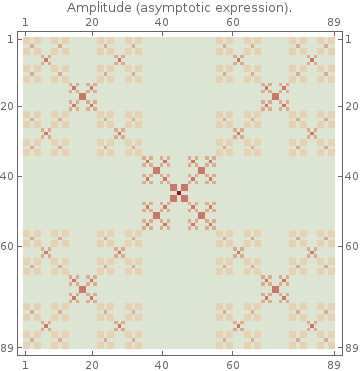
\includegraphics[width=.75\textwidth]{img/amplitude_asym.png}
  \caption{LDoS, asymptotic expression.}
  \label{fig:wf_idos_asym}
%\end{subfigure}%
%\begin{subfigure}{.5\textwidth}
  \centering
%  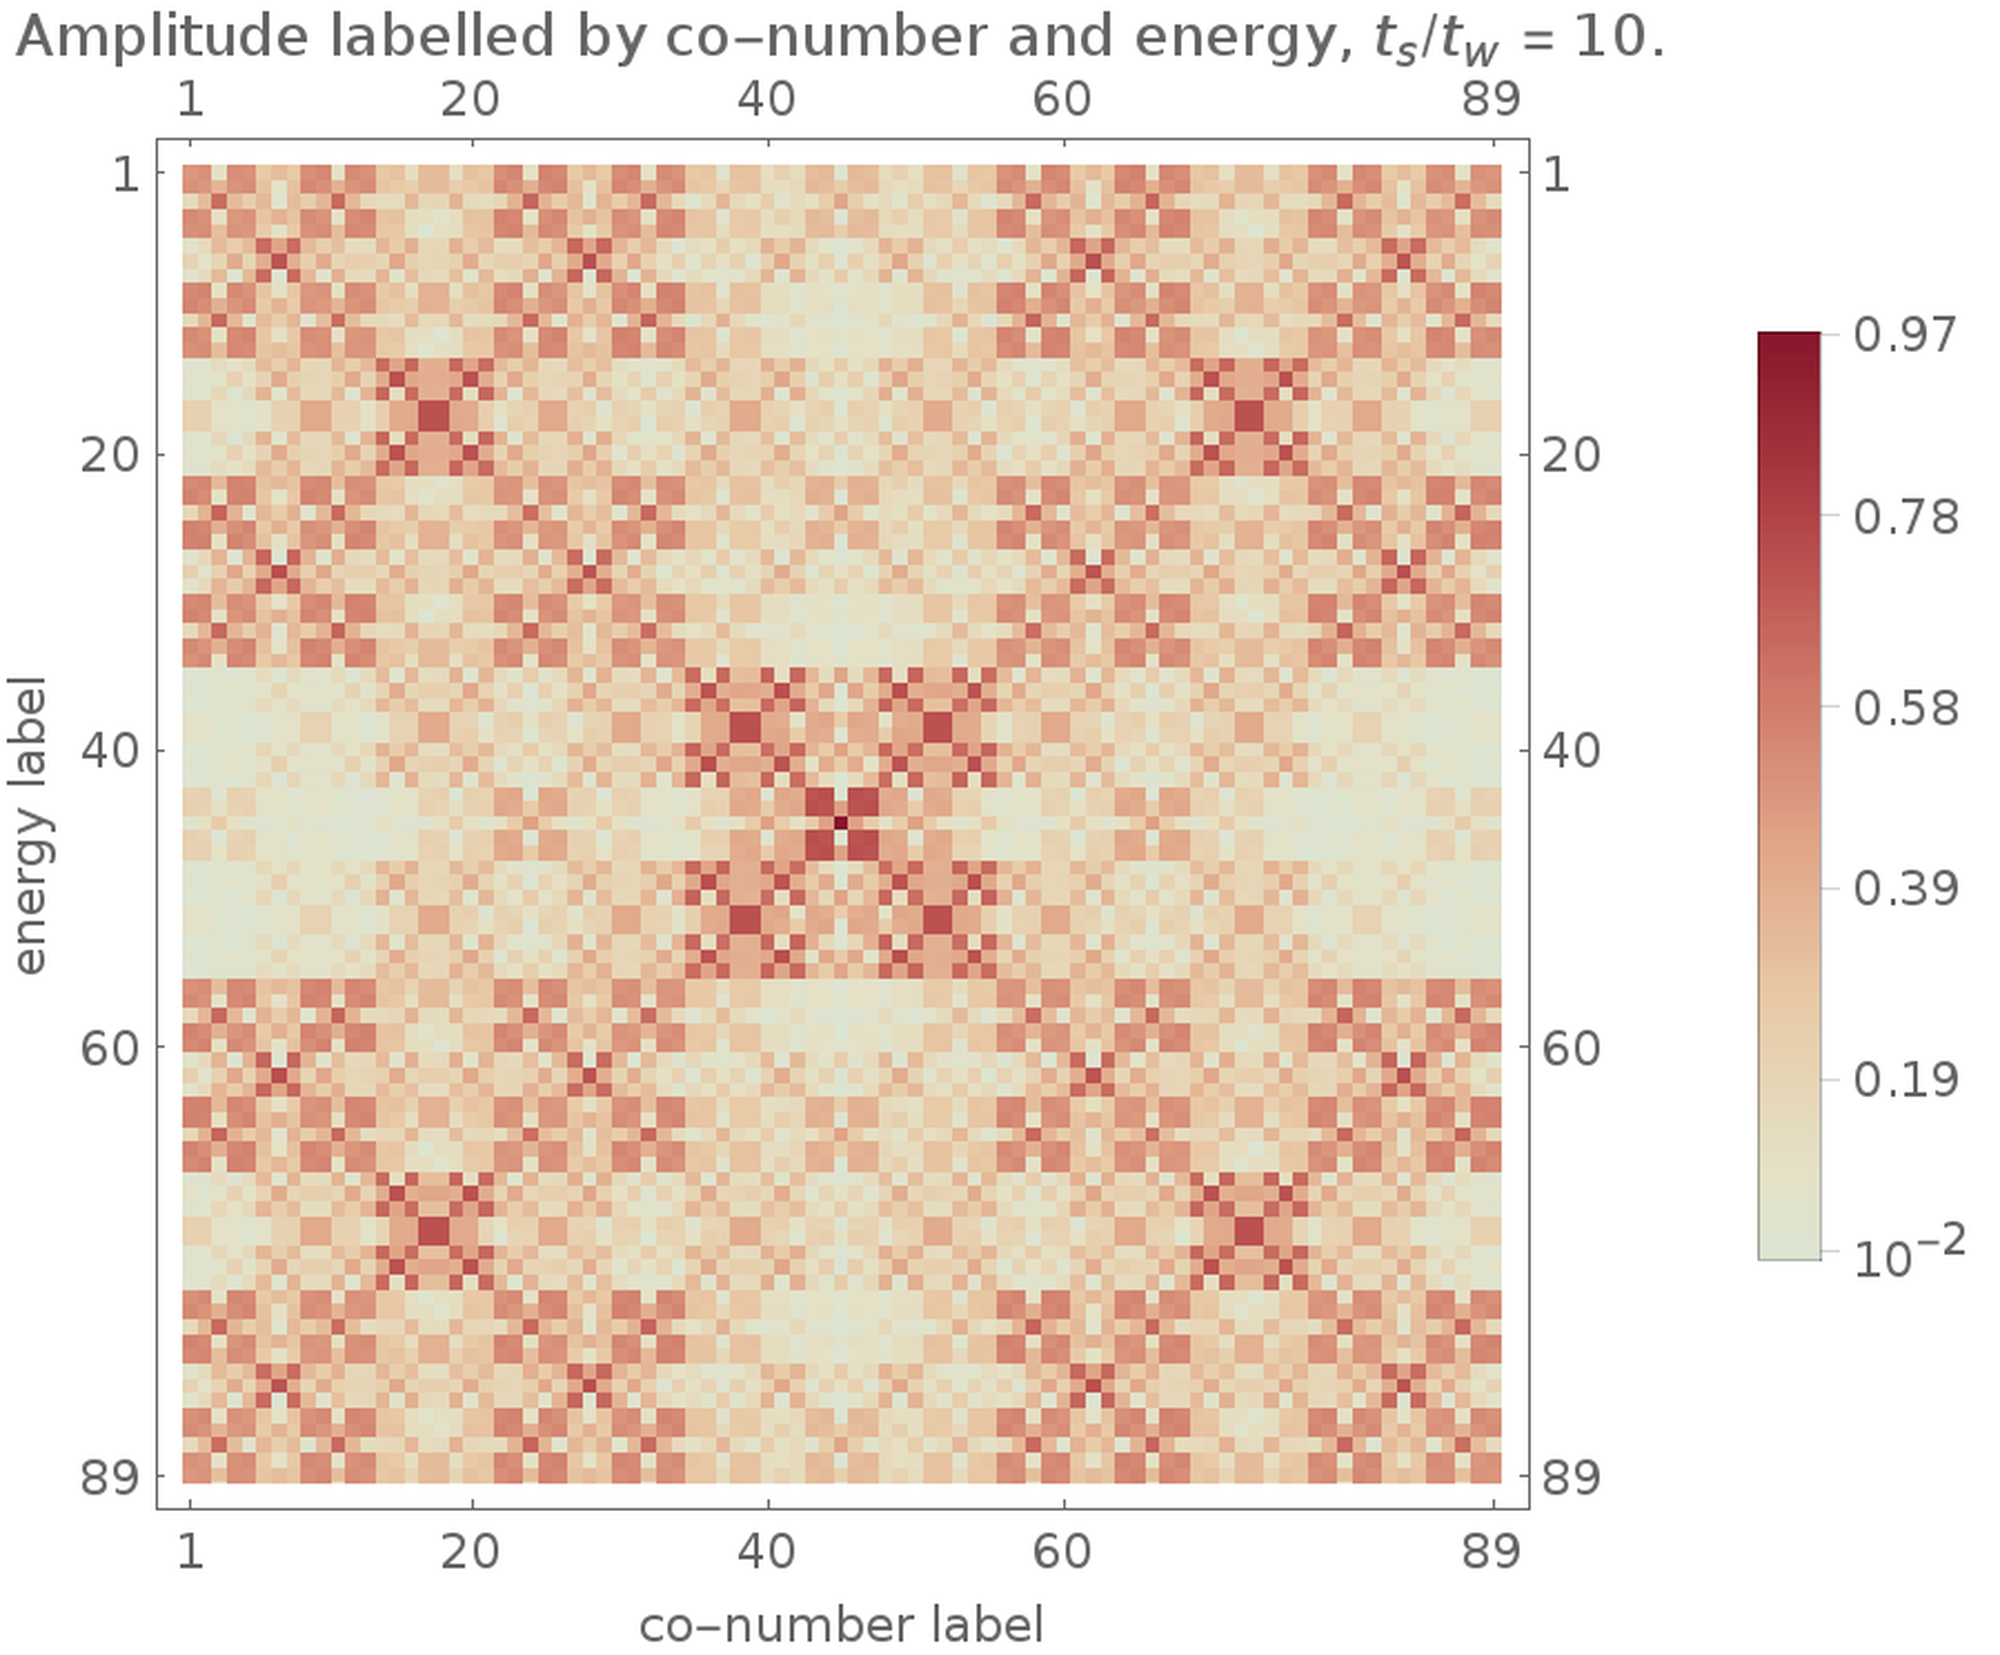
\includegraphics[width=1.\textwidth]{img/wf_idos.png}
  \caption{LDoS, numerical expression.}
  \label{fig:wf_idos_num}
%\end{subfigure} \\
\caption{The local density of states, as a function of the position label (in conumbering), and of the energy label, for the eigth approximant constituted of 89 sites.}
\label{fig:wf_idos}
\end{figure}

In conclusion, we have completely characterized the eigenstates of the $n^\text{th}$ approximant, and shown the equivalence between renormalization paths of sites and of energy levels. In the conumbering scheme, this equivalence becomes particularly simple. Recall,
 the first and the last $F_{n-2}$ sites of the $n^\text{th}$ approximant are molecular (bonding or antibonding) sites, while the remaining $F_{n-3}$ middle sites are atomic. 
Repeating this reasoning recursively: amongst the first $F_{n-2}$ sites, the first and last $F_{n-4}$ sites are molecular at step $n-2$, etc. 
Thus, in conumbering, sites are naturally ordered by their renormalization path, and the ordering is exactly the same as the one of the energy levels. As a result, plotting the local density of states as a function of the energy label and the site conumber, should make obvious the equivalence between renormalization paths of sites and of energy levels. In other words, the local density of states should be  {\it  invariant under the exchange of the site label and the energy label axes}. This is indeed what we observe, both analytically \eqref{fig:wf_idos_asym} and numerically for small values of $\rho$ \eqref{fig:wf_idos_num}.
xxxxxxxxxxxx ``We should point out that the inflation property has been used in \cite{thiem,repetowicz} to calculate wavefunctions in the strong modulation limit....etc etc''


\section{Fractal dimensions at leading order}
Now that we have completely characterized the spectrum and the wavefunction to leading order in $\rho$, we turn to the question of the fractal dimensions of the spectrum and of the wavefunctions.

\subsection{Fractal dimensions of the spectrum}

Fractal dimensions of the spectrum will be determined using the thermodynamical formalism \cite{Halsey1986}. We define the partition function
\begin{equation}
	\Gamma^n(q,\tau) = \sum_{a} \frac{\left( 1/F_n \right)^q}{(\Delta_a^n)^\tau}
\end{equation}
where $\Delta_a^n$ is taken to be the width of the energy band associated to the energy level labelled $a$.
One can show \cite{Halsey1986} that the generalized fractal dimensions of the spectrum $D_q$ are given by $D_q = \tau_q/(q-1)$ where $\tau_q$ is defined by
\begin{align}
	\Gamma^n(q,\tau > \tau_q) &\rightarrow +\infty \\
	\Gamma^n(a,\tau < \tau_q) &\rightarrow 0
\end{align}
In practice, a good approximation of $\tau_q$ is given by $\Gamma^{n+1}(q,\tau_q)/\Gamma^n(q,\tau_q) = 1$ for $n$ large.

In particular, we recall that the Hausdorff dimension, $D_0$, helps to characterize the nature of the spectrum. 
$D_0 = 0$ for a pure-point spectrum, while $D_0 = 1$ indicates that the spectrum has an absolutely continuous component.
An intermediate value $0 < D_0 < 1$ is the signature of a fractal spectrum.  Multifractal properties can be probed, finally, by varying $q$.

At leading order, the recursion relation between energies \eqref{eq:recur_spectrum} translates into a recursion relation between partition functions. This makes it easy to find the fractal dimensions of the spectrum \cite{Piechon95} \emph{via} the implicit equation
\begin{equation}
	2 \omega^{2 q} z^{-(q-1)D_q}+\omega^{3 q} \zb^{-(q-1)D_q} = 1.
\end{equation}
Thus, we have
\begin{equation}
	D_q = \frac{1}{1-q} \frac{\log \big[\omega^{-q} \left( \sqrt{1+\omega^{-q}} -1\right) \big]}{\log \rho} + \mathcal{O}\left( \frac{1}{(\log \rho)^2} \right)
\end{equation}
In particular, we find for the Hausdorff dimension
\begin{equation}
	D_0 = \frac{\log( \sqrt{2} -1 )}{\log \rho} + \mathcal{O}\left( \frac{1}{(\log \rho)^2} \right)
\end{equation}
in agreement with the result of Damanik \& Gorodetski \cite{DamanikGorodetski}, using trace-map-based methods.

We have $0 < D_0 < 1$ for $\rho > 0$. 
Therefore we recover the well-established result that the spectrum of the Fibonacci hamiltonian is fractal as soon as $\rho > 0$.

\subsection{Fractal dimensions of the wavefunctions}

The fractal dimensions $D_q(a)$ of the wavefunction associated to the energy level $a$ are defined by
\begin{equation}
	\chi_q^n(a) = \sum_i |\psi_i^n(a)|^{2q} \simlim{n}{\infty} \left( \frac{1}{F_n} \right)^{(q-1)D_q(a)}
\end{equation}
Note that $\chi_2(a)$ is the inverse participation ratio, and the exponent $D_2$ provides information as to the degree of localization of the state.The value $D_2(a) = 1$ indicates that the state $a$ is extended, while $D_2(a) = 0$ characterizes a localized state.
An intermediate value $0 < D_2(a) < 1$ is the signature of a critical state, whose multifractal properties can be probed by varying $q$.

At leading order in $\rho$ the renormalization of the eigenstates is trivial. 
On a site whose renormalization path matches the one of the energy level we consider, the amplitude at step $n$ is just the amplitude at step $n-3$ if the energy is in the atomic cluster, while the amplitude is the one at step $n-2$ divided by a factor $\sqrt{2}$ if the energy is in the molecular cluster.

Therefore, we have for the fractal dimensions of the wavefunction of the energy level labelled by $a$,
\begin{equation}
\label{eq:dqpsi0}
	D_q(a) = x_a \frac{\log 2}{\log \omega^{-1}} + \mathcal{O}(\rho^2),
\end{equation}
where
\begin{equation}
	x_a = \lim_{n \rightarrow \infty} \frac{n_+(a)+n_-(a)}{n}
\end{equation}
with $n_\pm(a)$ the number of $+$/$-$ letters in the renormalization path of $a$, i.e. $x_a$ is the fraction of RG steps in which the level $a$ corresponds to a molecular cluster.

Since $x_a \leq 1/2$, we have $0 < D_q(a) < 1$: the wavefunctions are critical, as we expect for a quasiperiodic system.
We have $x_a = 0$ for the level that has the renormalization path $00...$, ie for the energy level $E=0$, at the center of the atomic cluster. The corresponding eigenstate has a zero fractal dimension, and is thus completely localized. As we approach the $E=0$ level, $x_a$ approaches $0$ monotonically and the wavefunctions becomes more and more localized. This property has been observed in numerical calculations  \cite{thiem}....
The maximal value of $x_a=\frac{1}{2}$ is reached for the levels $E=E_\text{min}, E_\text{max} = \pm 1/(1+z)$ at the edges of the spectrum, for which the renormalization paths are $++...$ and $--...$.
The corresponding eigenstates are the most extended. They occupy a fraction $(1/F_n)^{\frac{\log 2}{\log \omega^{-2}}}$ of the sites.

To conclude, we note that, to leading order in $\rho$, the fractal dimensions of the wavefunction do not depend on $q$. Thus the wavefunctions are not multifractal at this order in $\rho$, and multifractality appears only at the next-to-leading order, which is discussed next.

\section{Fractal dimensions at next-to-leading order and multifractality}

To go beyond the leading order -- where the interesting physics lies! -- we must consider overlap between atoms and molecules. 
At next-to-leading order the picture of molecular and atomic eigenstates and energies remains relevant, but it is now possible for an ``atomic eigenstate'' to have nonzero amplitude on molecular sites, and vice-versa.
In this section devoted to the fractal dimensions, we find the corrections to the wavefunction amplitudes at next to leading order for the subset of sites considered in the previous section. This is sufficient for our purposes, and a complete analysis in perturbation theory to the next order is unnecessary.

We choose to write corrections to leading order via a multiplicative factor as follows:
\begin{equation}
	\psi_i^n(a) = \sqrt{\lambda_{ia}} \psi^{n}_{i,0}(a),
\end{equation}
where $\psi_{0}$ is the wavefunction at leading order. Note that $\psi^{n}_{i,0}(a)$ is related by the renormalization group to a wavefunction coefficient of a smaller approximant, with $\psi^{n}_{i,0}(a) = \psi^{n-3}_{i',0}(a')$ for an energy in the atomic cluster, and $ \psi^{n-2}_{i',0}(a')/\sqrt{2}$ for an energy in the molecular clusters. 

Introducing the average value $\lambda_a$, over all sites, but for fixed energy $E_a$, one can write
\begin{equation}
	\lambda_{ia} = \lambda_a + \Delta \lambda_{ia}.
\end{equation}
where we expect, in the spirit of perturbation theory, fluctuations around the average value to be small for $\rho$ small. Indeed, numerically, we find the fluctuations $\Delta \lambda_i(a)$ to be negligible relative to the mean value. More precisely, we have
\begin{equation}
	\lambda_a^q \gg \lambda_a^{q-k} \Delta \lambda_{ia}^k, \text{~} \forall k \in [1,q]
\end{equation}
so that the validity of the approximation improves as $q$ becomes larger.

This means that, for $q \geq 1$, we can write
\begin{equation}
%	\chi_q^n(a) = \begin{cases*}
%	\lambda(a)^q \chi_q^{n-3}(a') & if $a$ is an atomic level, \\
%	\left(\lambda(a)/2\right)^q \chi_q^{n-2}(a') & if $a$ is a molecular level. \\
%	\end{cases*}
\end{equation}
Iterating this recurrence relation, we find that 
\begin{equation}
\label{eq:rec_chi}
	\chi_q^n(a) = \left( \lambda_a \lambda_{a'}... \right)^q \chi_{q,0}^{n}(a).
\end{equation}
where $\chi_{q,0}^{n}(a)$ is the first order approximation of $\chi$.
The product $\lambda(a)\lambda(a')...$ encodes the next-to-leading order corrections to $\chi$, which are seen, thus, 
to depend only on the RG path of the energy level 

We next {\it assume} (as confirmed by numerical results) that the renormalization factor $\lambda(a)$ is constant over the atomic and the molecular clusters , i.e.
\begin{equation}
%	\lambda(a) = \begin{cases*}
%	\lb & if $a$ is an atomic level, \\
%	\lambda & if $a$ is a molecular level. \\
%	\end{cases*}
\end{equation}
The details of calculations for $\lb$ and $\lambda$ are given in the appendix \eqref{app:renorm}. We find
\begin{equation}
\label{eq:lamb}
%	\begin{cases}
		\lb = 1/(1+2\rho^2) + \mathcal{O}(\rho^4), \\
		\lambda = 1/(1+\rho^2/2) + \mathcal{O}(\rho^4).
%	\end{cases}
\end{equation}
Furthermore, the recurrence relation \eqref{eq:rec_chi} can be solved, and we find
\begin{equation}
	D_q(a) = D_q^{(0)}(a) - \frac{q}{q-1} \left( x_a \frac{\log \lambda}{\log \omega^{-1}} + \frac{1-2x_a}{3}\frac{\log \lb}{\log \omega^{-1}} \right).
\end{equation}
valid for any $\lb$ and $\lambda$.
Plugging in the values \eqref{eq:lamb}, we get the following expression correct to next to leading order
\begin{equation}
\label{eq:dqpsi2}
	D_q(a) = D_q^{(0)}(a) + \frac{q}{q-1} \frac{4-5x}{6} \frac{\rho^2}{\log \omega^{-1}} + \mathcal{O}(\rho^4).
\end{equation}
This shows explicitly the $q$-dependence, and therefore  the multifractality of the wavefunctions.


%\bibliographystyle{apsrev}
%\bibliography{fibonacci}

\end{document} 